\documentclass{beamer}
\usepackage{graphicx}
\usepackage{listingsutf8}
\usepackage{mathtools}
\usepackage{appendixnumberbeamer}
\usepackage{pgfplots}
\usepackage{mathtools}
\pgfplotsset{compat=newest}
\lstset{basicstyle=\ttfamily,breaklines=true}
\graphicspath{ {../images/} }
\usetheme{metropolis}
\setbeamertemplate{footline}[frame number]
\setbeamertemplate{footline}[appendixframenumber]

\begin{document}

\title{Étude de couvertures de réseaux de métro, application de 
l'homologie persistante et optimisation.}
\author{Elowan ; 10381}
\date{\today}

\maketitle

\begin{frame}
    \frametitle{Trouver les zones les moins biens desservies par un réseau de métro}    
    Les principales étapes : 
    \itemize{
        \item \textit{Convertir} les données géographiques en espace métrique ;
        \item Créer une suite de formes géométriques à partir de cet espace ;
        \item Trouver les trous de ces formes.
    }

    \begin{figure}
        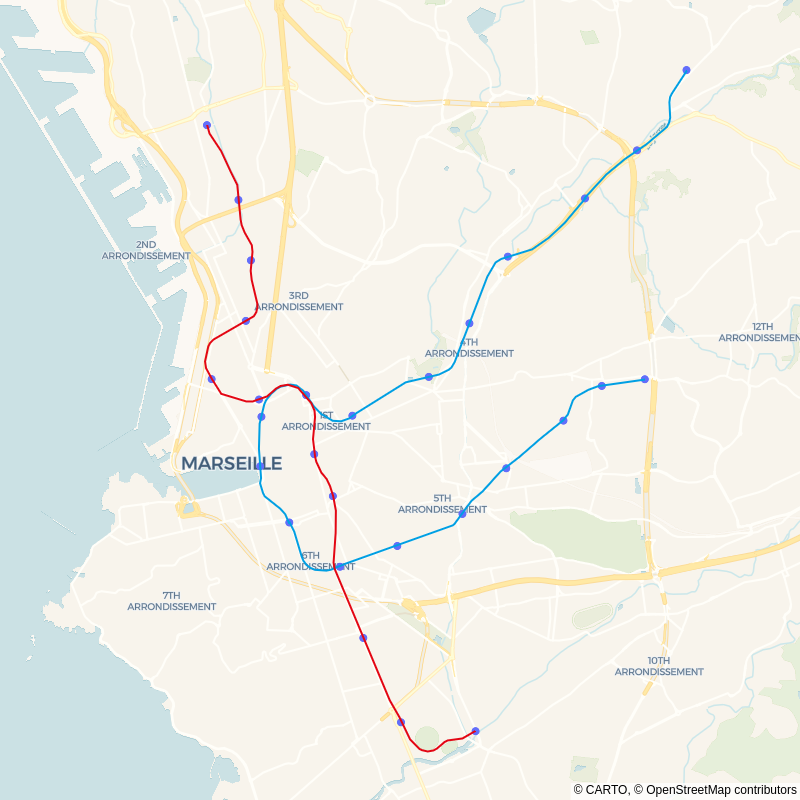
\includegraphics[width=0.4\textwidth]{../images/marseille_blank.png}
        \hfill
        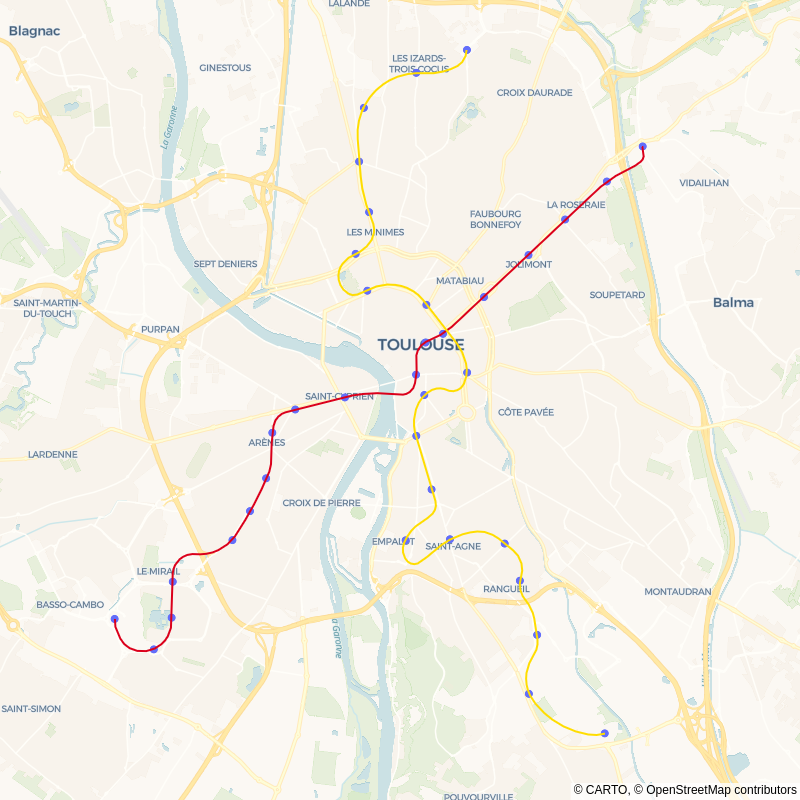
\includegraphics[width=0.4\textwidth]{../images/toulouse_blank.png}
        \centering
        \caption{Lignes de métros (Marseille et Toulouse)}
    \end{figure}
    
    
\end{frame}

\begin{frame}
    \frametitle{Plus en détail, reconnaitre un trou : l'idée du lasso}
    Chercher à enrouler au lasso, puis reduire ces lassos sans jamais le rompre ou déchirer la forme.  
    \begin{figure}
        \begin{tikzpicture}
            % \begin{axis}[
            %     axis equal image,
            %     axis lines=middle,
            %     xmax=18,zmax=5,
            %     ticks=none,
            %     clip bounding box=upper bound,
            %     colormap/blackwhite
            %     ]

            %     \addplot3[domain=0:360,y domain=0:320, samples=50,surf,z buffer=sort]
            %     ({(12 + 3 * cos(x)) * cos(y)} ,
            %     {(12 + 3 * cos(x)) * sin(y)},
            %     {3 * sin(x)});
            % \end{axis}
        \end{tikzpicture}
        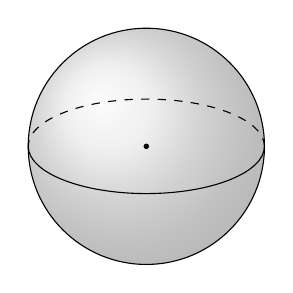
\begin{tikzpicture}
            \shade[ball color = gray!40, opacity = 0.4] (0,0) circle (1.5cm);
            \draw (0,0) circle (1.5cm);
            \draw (-1.5,0) arc (180:360:1.5 and 0.6);
            \draw[dashed] (1.5,0) arc (0:180:1.5 and 0.6);
            \fill[fill=black] (0,0) circle (1pt);
        \end{tikzpicture}
        \centering
        \caption{Un tore contenant deux trous et une sphère contenant 0 trou.}
    \end{figure}
\end{frame}

\begin{frame}
    \frametitle{Définitions}
    \begin{block}{Simplexe}
        Un simplexe $\sigma$ de dimension $k$ (ou $k$-simplexe) correspond à l'enveloppe convexe de $k+1$ vecteurs non inclus dans un sous-espace affine de dimension $k-1$.
    \end{block}

    \begin{block}{Face}
        On dit que $\sigma_i$ est une face de $\sigma_j$ si et seulement si $\sigma_i \subset \sigma_j$ et la dimension de $\sigma_i$ dim$(\sigma_i)$ est égale à dim$(\sigma_j) - 1$.
    \end{block}

    \begin{block}{Complexe simplicial}
        Un ensemble de simplexes.
    \end{block}

    \begin{figure}
        
\includegraphics[width=0.2\textwidth]{../images/SimpFaceCompl.png}
        \centering
        \caption{Exemple de complexe simplicial}
    \end{figure}
    
\end{frame}

\begin{frame}
    \frametitle{Définitions}
    \begin{block}{Filtration}
        Suite croissante pour l'inclusion de complexes simpliciaux.
    \end{block}

    \begin{figure}
        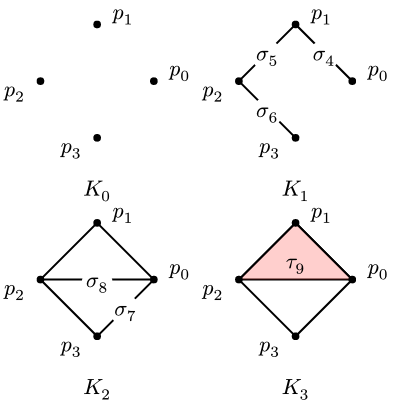
\includegraphics[width=0.5\textwidth]{../images/filtration_ex.png}
        \centering
        \caption{Exemple de filtration.}
    \end{figure}
\end{frame}
\begin{frame}
    \frametitle{Définitions}
    \begin{block}{Classe d'homologie}
        Elle représente un trou en dimension $n$.
    \end{block}

    \begin{figure}
        \centering
        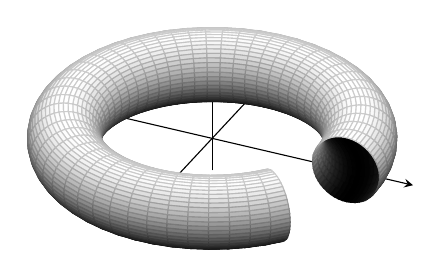
\begin{tikzpicture}
            \begin{axis}[
                axis equal image,
                axis lines=middle,
                xmax=18,zmax=5,
                ticks=none,
                clip bounding box=upper bound,
                colormap/blackwhite
                ]

                \addplot3[domain=0:360,y domain=0:320, samples=50,surf,z buffer=sort]
                ({(12 + 3 * cos(x)) * cos(y)} ,
                {(12 + 3 * cos(x)) * sin(y)},
                {3 * sin(x)});
            \end{axis}
        \end{tikzpicture}
        \hfill
        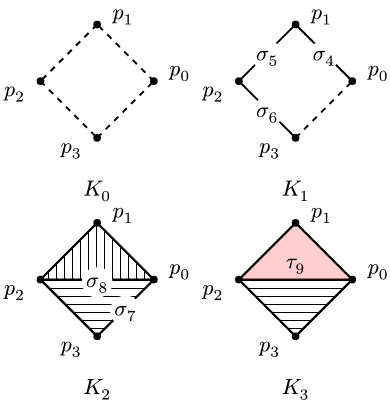
\includegraphics[width=0.4\textwidth]{../images/filtrationHomo.png}
        \caption{Le tore avec ces deux classes d'homologies et la filtration d'exemple avec en pointillé les classes d'homologies de dimension 0 et en hachuré celles de dimension 1.}
    \end{figure}
\end{frame}

\begin{frame}
    \frametitle{La méthode de l'homologie persistante}
    \itemize{
        \item Construire une filtration à partir d'un ensemble de points ;
        \item Application de l'algorithme \textit{standard} ;
        \item Récupération des classes d'homologies.
    }

    \begin{figure}
        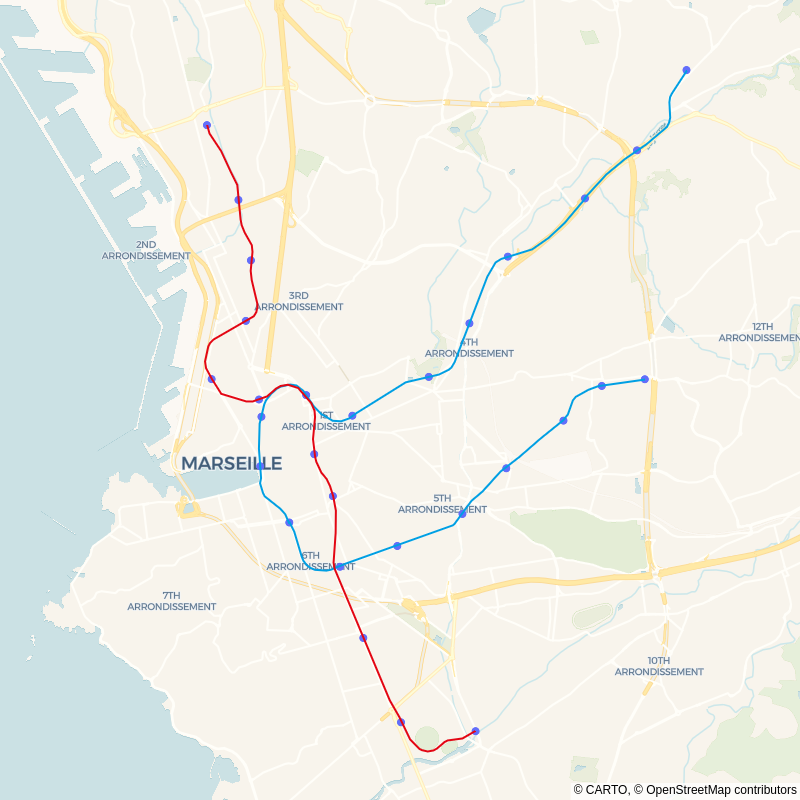
\includegraphics[width=0.4\textwidth]{../images/marseille_blank.png}
        \hfill
        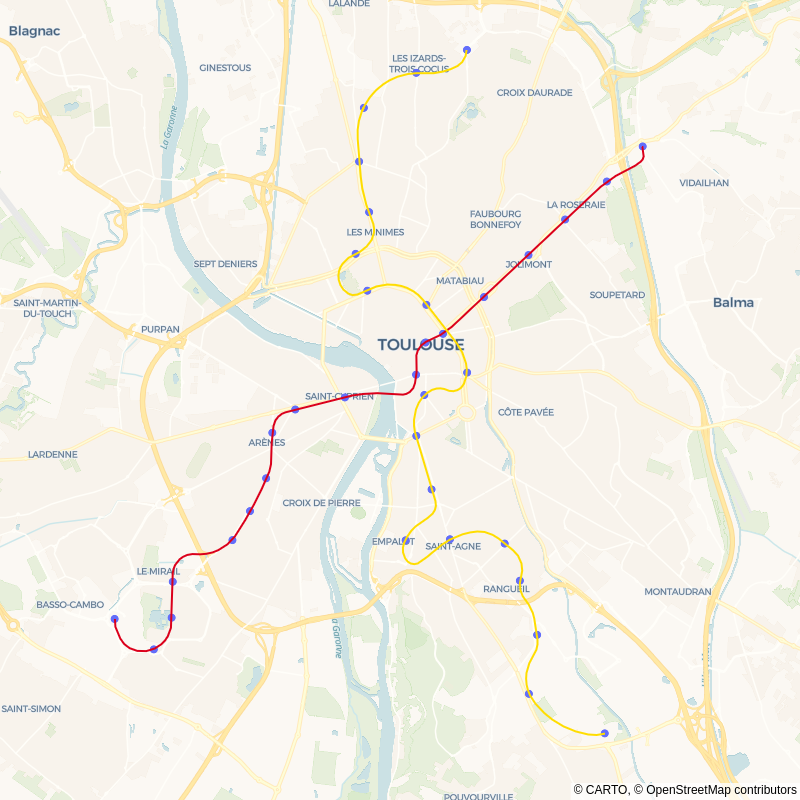
\includegraphics[width=0.4\textwidth]{../images/toulouse_blank.png}
        \centering
        \caption{Lignes de métros (Marseille et Toulouse)}
    \end{figure}

\end{frame}

\begin{frame}
    \frametitle{Définition de la distance}
    
    \begin{block}{Distance}
        On définit la distance $d$ entre deux stations de metro $x$ et $y$ : 
        $$ d(x,y) = \frac{1}{2}(min(t_{pied}(x,y), t_{voit}(x,y)) + min(t_{pied}(y,x), t_{voit}(y,x)))$$
    \end{block}

    \begin{block}{Poids d'une station}
        La moyenne sur une semaine du temps d'attente en station.
    \end{block}
\end{frame}

\begin{frame}
    \frametitle{Définition des complexes pondérés de Vietoris-Rips}
    \begin{block}{Complexe Simplicial pondéré de Vietoris-Rips}
        On le définit au rang $r$, comme l'ensemble des simplexes $(x_{i_0}, ..., x_{i_k})$ tels que : 
        $$
            \begin{cases}
                \forall j \in [|0, k|], poids_{i_j} < r\\
                \forall (j,l) \in [|0, k|]^2, d(x_{i_j}, x_{i_l}) + poids_{i_j} + poids_{i_l} < 2r
            \end{cases}
        $$
    \end{block}

    \begin{figure}
        \centering
        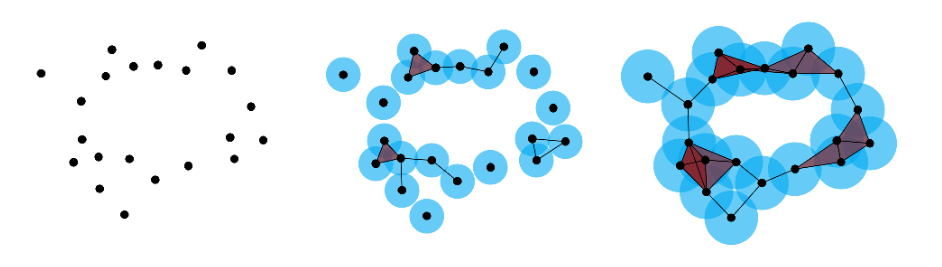
\includegraphics[width=0.8\textwidth]{../images/cech.png}
        \caption{Image repr les vietoris rips, tiré de \textit{Persitent homology for resource coverage: A case study of access to polling sites}}
    \end{figure}
    
\end{frame}

\begin{frame}
    \frametitle{Préparatif de l'algorithme (1/2): Ordre total sur les simplexes}
    Soient une filtration $K_0 \subset K_1 \subset ... \subset K_p$ et l'ensemble $S$ de tous les simplexes apparaissant dans la filtration. On indice $S$ de sorte que pour tout $\sigma_i$ et $\sigma_j$ de $S$: 

    $$ 
    \begin{rcases}
        \text{Si } \sigma_i \in K_{k_i} \text{ et } \sigma_j \in K_{k_j} \text{ avec } k_i < k_j\\
        \text{Sinon si } \sigma_i \text{ est une face de } \sigma_j
    \end{rcases}\Rightarrow i < j 
    $$
    L'ordre total est déduit de cet indiçage.
    \begin{figure}
        \centering
        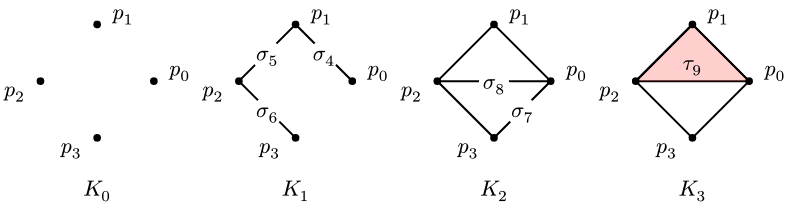
\includegraphics[width=0.8\textwidth]{../images/filtration_horizontal.png}
        \caption{Indiçage de la filtration}
    \end{figure}
\end{frame}


\begin{frame}
    \frametitle{Préparatif de l'algorithme (2/2): Matrice de bordure}
    \fontsize{8}{10}\selectfont
    \begin{figure}[h]
        \centering
        \begin{minipage}[c]{0.45\linewidth}
            \centering
            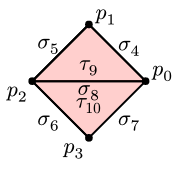
\includegraphics[width=0.6\textwidth]{"../images/notationSimplexe.png"} 
        \end{minipage}
        \hfill
        \begin{tabular}{ c | c | c | c | c | c | c }
                & 4 & 5 & 6 & 7 & 8 & 9 \\ \hline
            0   & 1 &   &   & 1 & 1 &   \\ \hline
            1   & 1 & 1 &   &   &   &   \\ \hline
            2   &   & 1 & 1 &   & 1 &   \\ \hline
            3   &   &   & 1 & 1 &   &   \\ \hline
            4   &   &   &   &   &   & 1 \\ \hline
            5   &   &   &   &   &   & 1 \\ \hline
            6   &   &   &   &   &   &   \\ \hline
            7   &   &   &   &   &   &   \\ \hline
            8   &   &   &   &   &   & 1 \\ \hline
            \textbf{low} & \textbf{1} & \textbf{2} & \textbf{3} & 
            \textbf{3} & \textbf{2} & \textbf{8}
        \end{tabular}
        
        \caption{Exemple de matrice de bordure $B$ associé à un ordre total}
    \end{figure}
\end{frame}


\begin{frame}[fragile]
    \frametitle{Application de l'algorithme}
    \begin{block}{Algorithme Standard($B \in M_n(\{0,1\})$)}
        \fontsize{9.5}{10}\selectfont
        \begin{lstlisting}
for j allant de 0 a n-1:
    while (il existe i < j avec low[i] = low[j]):
        ajouter colonne i de B a colonne j modulo 2
      \end{lstlisting}
    \end{block}
\end{frame}


\begin{frame}
    \frametitle{Compréhension du résultat en sortie}
    \begin{figure}
        \fontsize{6}{8}\selectfont
        \begin{math}
        \begin{array}{cc}
            \begin{tabular}{ c | c | c | c | c | c | c }
                  & 4 & 5 & 6 & 7 & 8 & 9 \\ \hline
                0 & 1 &   &   & 1 & 1 &   \\ \hline
                1 & 1 & 1 &   &   &   &   \\ \hline
                2 &   & 1 & 1 &   & 1 &   \\ \hline
                3 &   &   & 1 & 1 &   &   \\ \hline
                4 &   &   &   &   &   & 1 \\ \hline
                5 &   &   &   &   &   & 1 \\ \hline
                6 &   &   &   &   &   &   \\ \hline
                7 &   &   &   &   &   &   \\ \hline
                8 &   &   &   &   &   & 1 \\ \hline
                \textbf{low} & \textbf{1} & \textbf{2} & \textbf{3} & 
                \textbf{3} & \textbf{2} & \textbf{8}
            \end{tabular} & 
            \begin{tabular}{ c | c | c | c | c | c | c }
                  & 4 & 5 & 6 & 7 & 8 & 9 \\ \hline
                0 & 1 &   &   &   &   &   \\ \hline
                1 & 1 & 1 &   &   &   &   \\ \hline
                2 &   & 1 & 1 &   &   &   \\ \hline
                3 &   &   & 1 &   &   &   \\ \hline
                4 &   &   &   &   &   & 1 \\ \hline
                5 &   &   &   &   &   & 1 \\ \hline
                6 &   &   &   &   &   &   \\ \hline
                7 &   &   &   &   &   &   \\ \hline
                8 &   &   &   &   &   & 1  \\ \hline
                \textbf{low} & \textbf{1} & \textbf{2} & \textbf{3} & 
                \textbf{-1} & \textbf{-1} & \textbf{8}
            \end{tabular}
        \end{array}
        \end{math}
        \caption{Matrice $B$ et réduite $\overline{B}$}
    \end{figure}
    \begin{figure}
        \centering
        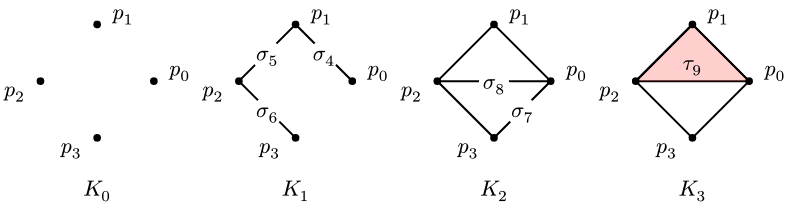
\includegraphics[width=0.7\textwidth]{../images/filtration_horizontal.png}
        \caption{Filtration et utilisée}
    \end{figure}
\end{frame}

\begin{frame}
    \frametitle{Optimisation}
    Remarques à l'initiative de la recherche d'optimisation :
    \begin{itemize}
        \item La matrice est creuse ;
        \item L'opération de somme de colonnes laisse invariante tous les simplexes de dimension différente.
    \end{itemize}

    Modifications apportées :
    \begin{itemize}
        \item Représentation de la matrice en liste d'adjacence (double liste chaînée ordonnée) ;
        \item Application de l'algorithme sur des matrices extraites et non la totale.
    \end{itemize}
\end{frame}

\begin{frame}[fragile]
    \frametitle{Algorithme optimisé}
    \begin{block}{Algorithme Standard optimisé($B \in M_n(\{0,1\})$)}
        \fontsize{9.5}{10}\selectfont
        \begin{lstlisting}
dims <- Tableau des simplexes ou dims[i] contient la liste des simplexes de dimension i
for toute dimension d a considerer:
    for chaque simplexe j de dims[d]
        while (il existe i dans dims[d] tel que low[j] = low[i]):
            ajouter colonne i de B a colonne j modulo 2
      \end{lstlisting}
    \end{block}
\end{frame}

\begin{frame}
    \frametitle{Résultats}
    \begin{figure}%
        \centering
        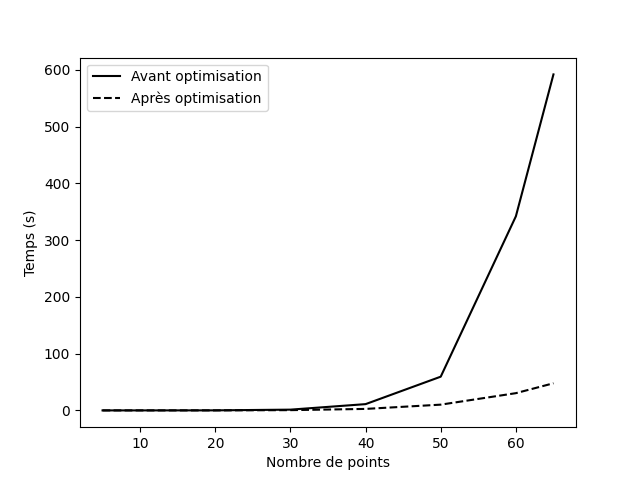
\includegraphics[width=0.8\textwidth]{../images/analyse_cmpx.png}
        \caption{Ordonnée linéaire}
    \end{figure}
\end{frame}

\begin{frame}
    \frametitle{Résultats}
    \begin{figure}%
        \centering
        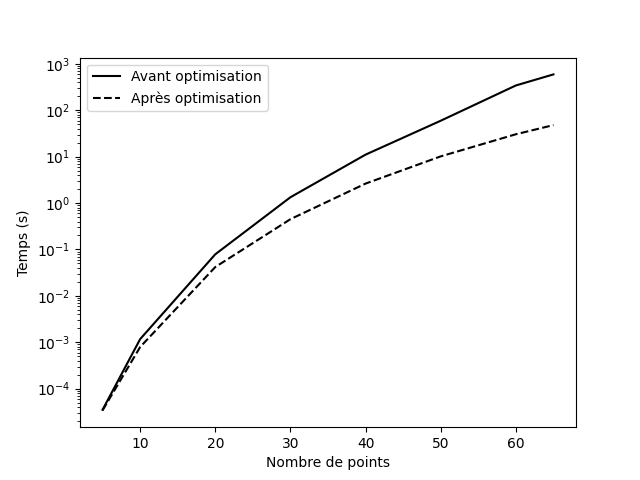
\includegraphics[width=0.8\textwidth]{../images/analyse_cmpx_log.png}
        \caption{Ordonnée logarithmique}
    \end{figure}
\end{frame}


\begin{frame}
    \frametitle{Résultats}
    \begin{figure}[h]
        \centering
        \begin{minipage}[c]{.42\linewidth}
            \centering
            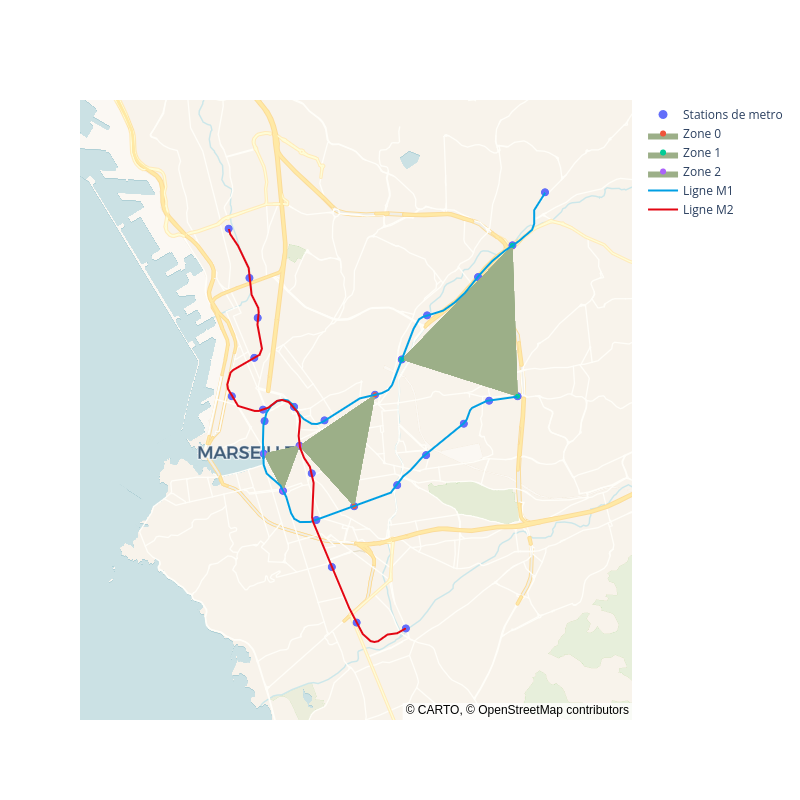
\includegraphics[width=1.1\textwidth]{../../Code/images/marseille.png}
            \caption{Marseille}
        \end{minipage}
        \hfill
        \begin{minipage}[c]{.42\linewidth}
            \centering
            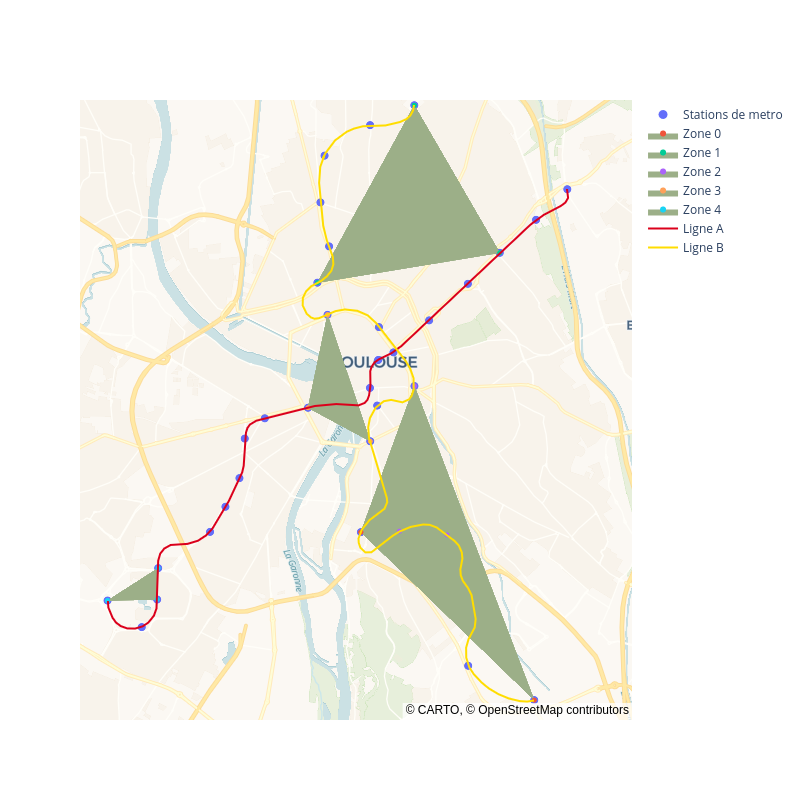
\includegraphics[width=1.1\textwidth]{../../Code/images/toulouse.png}
            \caption{Toulouse}
        \end{minipage}
    \end{figure}
\end{frame}

\appendix

\begin{frame}
    \frametitle{Annexe : Définition}
    \begin{block}{Complexe de chaînes}
        On définit un \textit{complexe de chaînes} comme la donnée d'une suite 
    
        $$... \xrightarrow{\delta_{k+2}} C_{k+1} \xrightarrow{\delta_{k+1}} C_k \xrightarrow{\delta_k} C_{k-1} \xrightarrow{\delta_{k-1}} ...$$

        Où chaque $C_k$ est un groupe abélien libre qui a pour base les $k$-simplexes de $X$ et $\delta_k$ est une morphisme de groupes tel que $\delta_k \circ \delta_{k+1} = 0$
        
        On appelle $\delta_k$ un \textit{opérateur de bords}.

    \end{block}
    \begin{block}{Classes d'homologies $H_k$}
    On définit alors les \textit{classes d'homologie de dimension $k$} comme le groupe de $Ker(\delta_k)$ quotienté par $Im(\delta_{k+1})$:

    $$H_k = Ker(\delta_k) / Im(\delta_{k+1})$$
    \end{block}
\end{frame}

\begin{frame}
    \frametitle{Annexe : Théorème des facteurs invariants}
    Il existe un unique ensemble ${d_1, ..., d_p}$ d'éléments de $H_k$ définis à des inversibles près, tel que :
    $$H_k (X) \simeq \bigoplus_{i=1}^p P_k (X) / d_i P_k (X)$$

    en notant $P_k(X)$ l'ensemble des parties à $k+1$ éléments de X, formant donc un complexe simplicial constitué uniquement de $k$-simplexes. Cet ensemble est appelé \textit{code barre} de $H_k$.
\end{frame}

\begin{frame}
    \frametitle{Annexe : Diagrammes de persistance}
    % \begin{figure}
    %     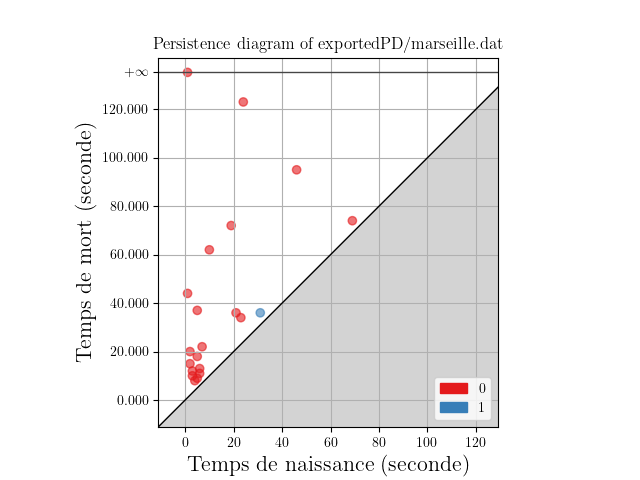
\includegraphics[width=0.7\textwidth]{pd_marseille}
    %     \centering
    %     \caption{Diagramme de persistance}
    % \end{figure}

    \begin{figure}[h]
        \centering
        \begin{minipage}[c]{.45\linewidth}
            \centering
            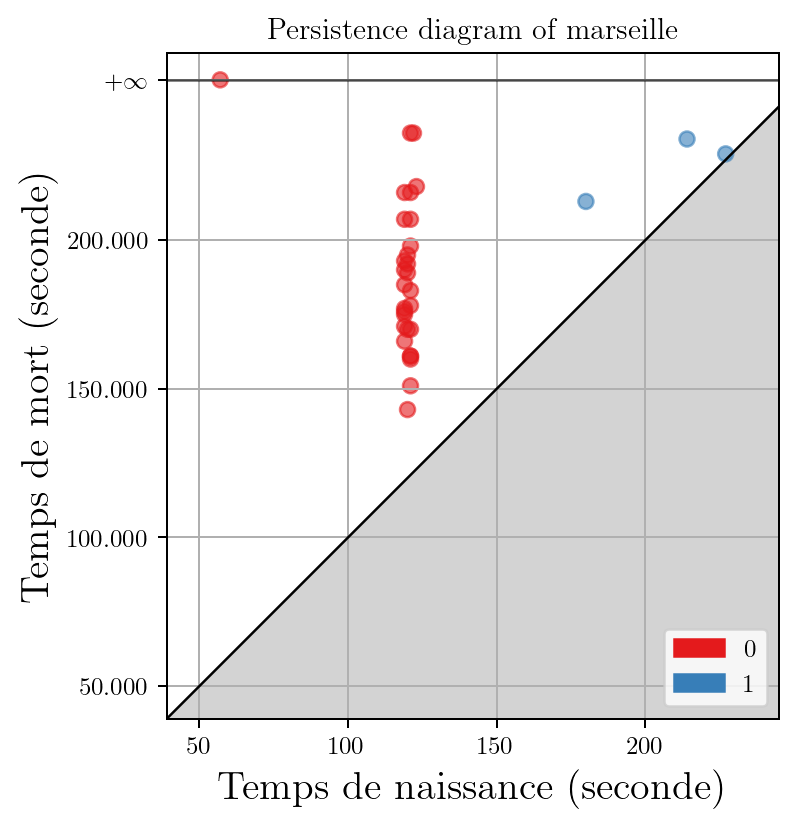
\includegraphics[width=1\textwidth]{../../Code/images/pd_marseille.png}
            \caption{Diagramme de persistance de Marseille}
        \end{minipage}
        \hfill
        \begin{minipage}[c]{.45\linewidth}
            \centering
            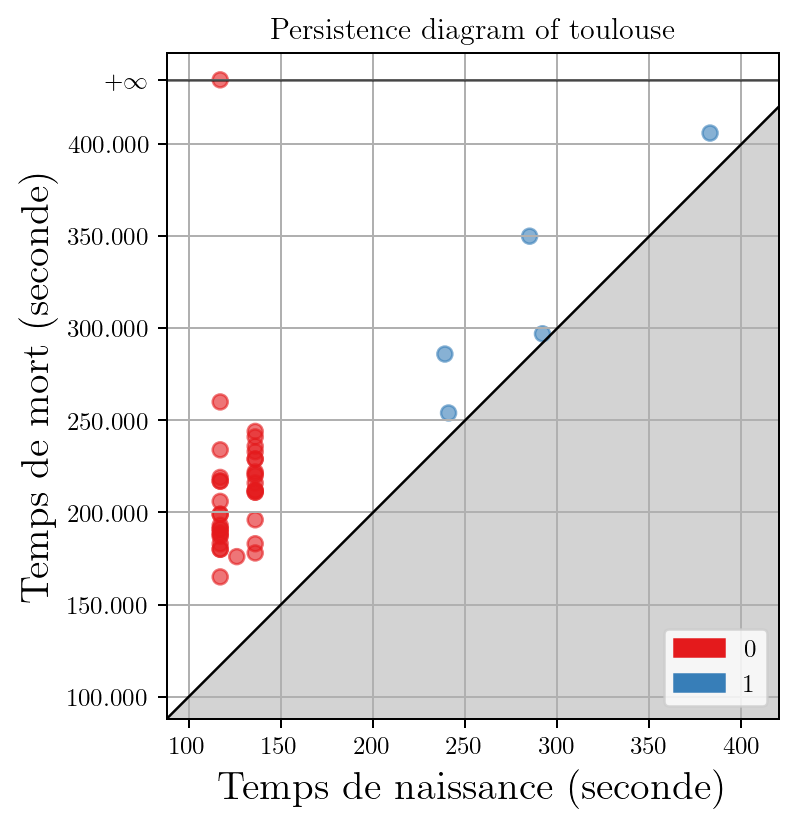
\includegraphics[width=1\textwidth]{../../Code/images/pd_toulouse.png}
            \caption{Diagramme de persistance de Toulouse}
        \end{minipage}
    \end{figure}
\end{frame}

\begin{frame}
    \frametitle{Annexe : Récupération des données}
    Pour le calcul des temps de trajet :  apidocs.geoapify.com

    Pour la récupération des stations et des temps d'attentes moyens : transport.data.gouv.fr
\end{frame}
\end{document}